\documentclass[9pt]{beamer}
\usetheme{Warsaw}
\usefonttheme[onlymath]{serif}

\usepackage[utf8]{inputenc}
%\usepackage[polish]{babel}
\usepackage[T1]{fontenc}
\usepackage{comment}
\usepackage{setspace}
\usepackage{amsmath}
\usepackage{dcolumn}
\usepackage{siunitx}
\usepackage{tabularx}
\usepackage{graphicx}
\usepackage{algpseudocode}
\graphicspath{{../images/}}

\sisetup{
    table-number-alignment = center, % Align numbers at the decimal point
    table-format = +1.4e3,           % Specify number format: 1 digit before, 3 after decimal, and 1 exponent
    tight-spacing = true,           % Remove extra spacing around numbers
}

\newcolumntype{M}{>{\centering\arraybackslash\math}p{2cm}}

\newcommand{\n}{\newline}

\linespread{1}

\title{Projekt 1, Zadanie 23}
\author{Wiktor Murawski, 333255, grupa 3, środa 12:15}
\date{}

\begin{document}

\begin{frame}
    %\frametitle{\insertauthor,\space\inserttitle}

    \begin{spacing}{1.75}
    \begin{center}
        \inserttitle\par
        \insertauthor
    \end{center}
    \vspace{2em}
    Obliczanie całek $ \iint\limits_D f(x,y) \, dxdy $ na obszarze
    $  D = \{(x,y) \in \mathbb{R}^2 : |x| + |y| \leq 1\} $
    poprzez podział obszaru $ D $ na $ 4n^2 $ trójkątów przystających oraz
    zastosowanie na każdym z nich kwadratury rzędu drugiego.
    \end{spacing}
\end{frame}


\begin{frame}
\frametitle{Podział obszaru $D$ na $4n^2$ trójkątów przystających}
    \begin{columns}
        \column{0.5\textwidth}
        \centering
        Podział $D$ dla $n = 1$\\
        \vspace{1em}
        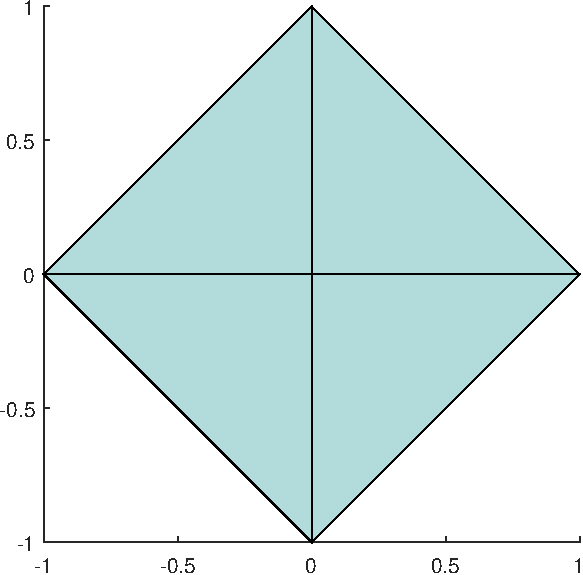
\includegraphics[width=\textwidth]{figure1.pdf}


        \column{0.5\textwidth}
        \centering
        Podział $D$ dla $n = 4$\\
        \vspace{1em}
        \includegraphics[width=\textwidth]{figure4.pdf}

    \end{columns}
\end{frame}


\begin{frame}
	\frametitle{Algorytm podziału}
	\begin{algorithmic}
		\For{$\mathtt{x = 0,1,2,...,n-1}$}
			\State $\mathtt{r \gets 1}$
			\For{$\mathtt{y = 0,0,1,1,...,n-x-2,n-x-2,n-x-1}$}
				\State $\mathtt{r \gets !r}$
				\State $\mathtt{(x_1,y_1) \gets (\dfrac{x+r}{n},\dfrac{y+r}{n})}$\\
				\State $\mathtt{(x_2,y_2) \gets (\dfrac{x+1}{n},\dfrac{y}{n})}$\\
				\State $\mathtt{(x_3,y_3) \gets (\dfrac{x}{n},\dfrac{y+1}{n})}$\\
				\State $\texttt{Oblicz współrzędne trójkątów w II, III i IV ćwiartce}$
				\vspace{0.5em}
				\State $\texttt{Zastosuj kwadraturę na wyznaczonych trójkątach}$
			\EndFor
		\EndFor
	\end{algorithmic}
\end{frame}

\begin{frame}
	\frametitle{Przykład działania algorytmu dla $n = 2$}
	\vspace{-1.5cm}
	\begin{columns}[T, onlytextwidth] % Create columns
		\begin{column}{0.5\textwidth} % First column takes half the width
			\begin{figure}
				\centering
				\includegraphics[width=\linewidth]{part1.pdf}
			\end{figure}
		\end{column}
		
		\begin{column}{0.5\textwidth} % Second column takes half the width
			\begin{figure}
				\centering
				\includegraphics[width=\linewidth]{part2.pdf}
			\end{figure}
		\end{column}
	\end{columns}
	\vspace{-3cm}
	\begin{columns}[T, onlytextwidth] % Another set of columns
		\begin{column}{0.5\textwidth} % Third column
			\begin{figure}
				\centering
				\includegraphics[width=\linewidth]{part3.pdf}
			\end{figure}
		\end{column}
		
		\begin{column}{0.5\textwidth} % Fourth column
			\begin{figure}
				\centering
				\includegraphics[width=\linewidth]{part4.pdf}
			\end{figure}
		\end{column}
	\end{columns}
\end{frame}


\begin{frame}
    \frametitle{Formuła całkowa na trójkącie}
    Niech $T$ będzie trójkątem o wierzchołkach $(x_1,y_1), (x_2,y_2), (x_3,y_3) \in \mathbb{R}^2$
    Niech $P$ oznacza pole trójkąta $T$ oraz niech 
    $$ A = \begin{pmatrix}
    	1 & 1 & 1 \\
    	x_1 & x_2 & x_3 \\
    	y_1 & y_2 & y_3 \\
    \end{pmatrix} $$
    Wtedy $$P = \frac{1}{2}|\det{A}|$$
    Niech $f : \mathbb{R}^2 \to \mathbb{R}$. Wówczas 
    $$S_S(f) = P f \left(\frac{x_1+x_2+x_3}{3},\frac{y_1+y_2+y_3}{3} \right) $$
    $$S_W(f) = \frac{P}{3} \Big( f(x_1,y_1) + f(x_2,y_2) + f(x_3,y_3) \Big)$$
    są kwadraturami rzędu 2-go.
    
\end{frame}

\begin{frame}
	 \begin{spacing}{1.5}
	Mając podział obszaru $ D $ na $4 n^2 $ trójkątów przystających oraz kwadraturę drugiego rzędu na dowolnym trójkącie, możemy obliczyć całkę $$ I(f) = \iint\limits_D f(x,y)  \, dxdy $$ poprzez zastosowanie na każdym z trójkątów kwadratury rzędu drugiego.\\
	
	Stosując kwadraturę $ S_S(f) $ na każdym z trójkątów, 
	otrzymamy kwadraturę złożoną, oznaczmy $ S_S^{[n]}(f) $.\\
   
    Metodę uznamy za poprawną, jeśli 
    $$ S_S^{[n]}(f) = I(f) $$
    dla $f$ będących wielomianami dwóch zmiennych stopnia $ < 2$. 
	W celu sprawdzenia poprawności metody przetestujemy ją na takich $f$ \par
	
%	Spodziewamy się, że dla dostatecznie dużego $ n $
%	$$ S_S^{[n]} \approx I(f) $$	
%	a dla wielomianów dwóch zmiennych stopnia $ < 2 $
%	$$ S_S^{[n]} = I(f) $$ 

	\end{spacing}
\end{frame}

\begin{frame}
\frametitle{Wyznaczenie analityczne całki z wielomianu stopnia 1}

    \begin{spacing}{1}
        Obliczymy analitycznie 
        $$ I = \iint\limits_D f(x,y) \, dx dy $$ 
        gdzie
        $$ f(x,y) = ax + by + c \qquad a,b,c \in \mathbb{R}$$
        Niech 
        $$ D_1 = \{(x,y) \in D : x \leq 0\} $$ 
        $$ D_2 = \{(x,y) \in D : x > 0\} $$ 
        Oznaczmy 
        $$ I_1 = \iint\limits_{D_1} f(x,y) \, dx dy $$ 
        $$ I_2 = \iint\limits_{D_2} f(x,y) \, dx dy $$ 
        Wtedy $ D = D_1 \cup D_2 $ oraz $ I = I_1 + I_2 $.
        %$$ I_1 = \int\limits_{-1}^{0}\int\limits_{-x-1}^{x+1} ax+by+c \, dy dx $$
        %$$ I_2 = \int\limits_{0}^{1}\int\limits_{x-1}^{-x+1} ax+by+c \, dy dx $$
    \end{spacing}

\end{frame}

\begin{frame}
\frametitle{Wyznaczenie analityczne całki z wielomianu stopnia 1}
    \begin{columns}
        \begin{column}{0.5\textwidth}
            % Lewa kolumna
            \begin{align*}
                I_1 &= \int\limits_{-1}^{0}\int\limits_{-x-1}^{x+1} ax+by+c \,dydx \\
                I_1 &= \int\limits_{-1}^{0}\left[axy + \frac{by^2}{2} + cy\right]_{-x-1}^{x+1} \,dx \\
                I_1 &= \int\limits_{-1}^{0} 2ax^2 + 2ax + 2cx + 2c \,dx \\
                I_1 &= 2\left[ \frac{ax^3}{3} + \frac{ax^2}{2} + \frac{cx^2}{2} + cx \right]_{-1}^{0} \\
                I_1 &= -\frac{a}{3} + c \\
            \end{align*}
        \end{column}
        \begin{column}{0.5\textwidth}
            % Prawa kolumna
            \begin{align*}
                I_2 &= \int\limits_{0}^{1}\int\limits_{x-1}^{-x+1} ax+by+c \,dydx \\
                I_2 &= \int\limits_{0}^{1}\left[axy + \frac{by^2}{2} + cy\right]_{x-1}^{-x+1} \,dx \\
                I_2 &= \int\limits_{0}^{1} - 2ax^2 + 2ax - 2cx + 2c \,dx \\
                I_2 &= 2\left[ -\frac{ax^3}{3} + \frac{ax^2}{2} - \frac{cx^2}{2} + cx \right]_{0}^{1} \\
                I_2 &= \frac{a}{3} + c \\
            \end{align*}
        \end{column}
    \end{columns}

    \begin{center}
        Ostatecznie otrzymujemy $ I = I_1 + I_2 = 2c $
    \end{center}
\end{frame}

\begin{frame}
	\frametitle{Testy poprawności}
	\begin{table}[]
		\makebox[\linewidth]{
			\begin{tabular}{|l|S|l|S|S|}
				\hline & & & & \\[-1em]
				Funkcja $f$  & {$ I(f) $} &{$n$}& {$S_S^{[n]}(f)$} & {$|S_S^{[n]}(f) - I(f)|$}\\
				\hline & & & &\\[-1em]
				%---------------------------------------------------------------------------				
$f(x,y) = $            & 2.0000e+00 & 1   & 2.0000e+00 & 0.0000e+00 \\%0.0000e+00
                       &            & 5   & 2.0000e+00 & 1.3323e-15 \\%6.6613e-16
$ 1 $			       &            & 10  & 2.0000e+00 & 2.0650e-14 \\%1.0325e-14
				       &            & 50  & 2.0000e+00 & 1.8763e-13 \\%9.3814e-14
				       &            & 100 & 2.0000e+00 & 2.0082e-12 \\%1.0041e-12
			           &            & 500 & 2.0000e+00 & 1.5836e-11 \\%7.9181e-12
				%---------------------------------------------------------------------------
				\hline & & & &\\[-1em]
				%---------------------------------------------------------------------------
$f(x,y) = $            & 2.0000e+00 & 1   & 2.0000e+00 & 0.0000e+00 \\%0.0000e+00
                       &            & 5   & 2.0000e+00 & 8.8818e-16 \\%4.4409e-16
$ x + y + 1 $	       &            & 10  & 2.0000e+00 & 2.4425e-15 \\%1.2212e-15
				       &            & 50  & 2.0000e+00 & 4.6629e-15 \\%2.3315e-15
				       &            & 100 & 2.0000e+00 & 4.8850e-15 \\%2.4425e-15
				       &            & 500 & 2.0000e+00 & 7.5939e-14 \\%3.7970e-14
				%---------------------------------------------------------------------------
				\hline & & & &\\[-1em]
$f(x,y) = $            & 1.0000e+00 & 1   & 1.0000e+00 & 0.0000e+00 \\%0.0000e+00
                       &            & 5   & 1.0000e+00 & 5.5511e-16 \\%5.5511e-16
$ 8x+2y+\frac{1}{2}$   &            & 10  & 1.0000e+00 & 2.2204e-16 \\%2.2204e-16
		               &            & 50  & 1.0000e+00 & 1.1102e-15 \\%1.1102e-15
	                   &            & 100 & 1.0000e+00 & 1.7764e-15 \\%1.7764e-15		    
	                   &            & 500 & 1.0000e+00 & 8.2157e-15 \\%8.2157e-15
				\hline
			\end{tabular}
		}
	\end{table}
\end{frame}

\begin{frame}
	\frametitle{Testy poprawności}
	\begin{table}[]
		\makebox[\linewidth]{
			\begin{tabular}{|l|S|l|S|S|}
				\hline & & & & \\[-1em]
				Funkcja $f$  & {$ I(f) $} &{$n$}& {$S_S^{[n]}(f)$} & {$|S_S^{[n]}(f) - I(f)|$}\\
				\hline & & & &\\[-1em]
				%---------------------------------------------------------------------------				
$ f(x,y) = $           &  2.8284e+00 & 1   &  2.8284e+00 & 0.0000e+00 \\%0.0000e+00  
                       &             & 5   &  2.8284e+00 & 1.3323e-15 \\%4.7103e-16  
$ x-y+\sqrt2$          &             & 10  &  2.8284e+00 & 1.7764e-15 \\%6.2804e-16  
                       &             & 50  &  2.8284e+00 & 5.3291e-15 \\%1.8841e-15  
                       &             & 100 &  2.8284e+00 & 3.0198e-14 \\%1.0677e-14  
                       &             & 500 &  2.8284e+00 & 1.5543e-14 \\%5.4953e-15  
				%---------------------------------------------------------------------------
				\hline & & & &\\[-1em]
				%---------------------------------------------------------------------------
$ f(x,y) = $           & -6.2832e+00 & 1   & -6.2832e+00 & 0.0000e+00 \\%-0.0000e+00  
                       &             & 5   & -6.2832e+00 & 8.8818e-16 \\%-1.4136e-16  
$ -x + 2y - \pi $      &             & 10  & -6.2832e+00 & 0.0000e+00 \\%-0.0000e+00  
                       &             & 50  & -6.2832e+00 & 3.5527e-15 \\%-5.6543e-16  
                       &             & 100 & -6.2832e+00 & 4.4409e-15 \\%-7.0679e-16  
                       &             & 500 & -6.2832e+00 & 3.5527e-14 \\%-5.6543e-15  
				%---------------------------------------------------------------------------
				\hline & & & &\\[-1em]
$ f(x,y) = $           &  0.0000e+00 & 1   &  0.0000e+00 & 0.0000e+00 \\%NaN  
                       &             & 5   &  1.3878e-17 & 1.3878e-17 \\%Inf  
$ \pi x - ey $         &             & 10  & -6.9389e-18 & 6.9389e-18 \\%Inf  
                       &             & 50  &  9.7578e-19 & 9.7578e-19 \\%Inf  
                       &             & 100 &  1.3281e-18 & 1.3281e-18 \\%Inf  
                       &             & 500 &  7.9028e-19 & 7.9028e-19 \\%Inf  
				\hline
			\end{tabular}
		}
	\end{table}
\end{frame}

\begin{frame}
	\frametitle{Testy numeryczne}
	\begin{spacing}{1.25}
		Przetestujemy teraz własności numeryczne zaimplementowanej metody. 
		Zaobserwujemy jak metoda działa dla kilku wybranych funkcji, które nie są wielomianami stopnia $ < 2 $.\\
		Zauważymy, że dla niskich $n$ wyniki są bardzo niedokładne. Intuicyjnie, im wyższe n, tym wyniki będą dokładniejsze; $k$-krotne zwiększenie wartości $n$ spowoduje około $k^2$-krotne zmniejszenie wartości błędu bezwzględnego.\\
		Wynika to z faktu wspomnianego na wykładzie, mianowicie jeśli $f$ jest wystarczająco wiele razy różniczkowalna, to 
		$$ | S^{[n]}(f) - I(f) | = \mathcal{O}(n^{-p})$$
		gdzie $p$ jest rzędem zastosowanej kwadratury, w naszym przypadku 
		$$ | S_S^{[n]}(f) - I(f) | = \mathcal{O}(n^{-2}) $$
	\end{spacing}
\end{frame}

\begin{frame}
	\frametitle{Testy numeryczne}
    \begin{table}[]
    	\makebox[\linewidth]{
    		\begin{tabular}{|l|S|l|S|S|}
    			\hline & & & & \\[-1em]
    			Funkcja $f$  & {$ I(f) $} &{$n$}& {$S_S^{[n]}(f)$} & {$|S_S^{[n]}(f) - I(f)|$}\\
    			\hline & & & &\\[-1em]
    			%---------------------------------------------------------------------------				
$ f(x,y) = $           &  6.6667e-01 & 1   &  4.4444e-01 & 2.2222e-01 \\%3.3333e-01  
                       &             & 5   &  6.5778e-01 & 8.8889e-03 \\%1.3333e-02  
$ (x+y)^2 $            &             & 10  &  6.6444e-01 & 2.2222e-03 \\%3.3333e-03  
                       &             & 50  &  6.6658e-01 & 8.8889e-05 \\%1.3333e-04  
                       &             & 100 &  6.6664e-01 & 2.2222e-05 \\%3.3333e-05  
                       &             & 500 &  6.6667e-01 & 8.8889e-07 \\%1.3333e-06      
    			%---------------------------------------------------------------------------
    			\hline & & & &\\[-1em]
    			%---------------------------------------------------------------------------
$ f(x,y) = $           &  4.0000e-01 & 1   & 1.9753e-01 & 2.0247e-01 \\%5.0617e-01  
                       &             & 5   & 3.8688e-01 & 1.3124e-02 \\%3.2810e-02  
$ (x+y)^4 $ 		   &             & 10  & 3.9668e-01 & 3.3202e-03 \\%8.3006e-03  
				       &             & 50  & 3.9987e-01 & 1.3331e-04 \\%3.3328e-04  
				       &             & 100 & 3.9997e-01 & 3.3332e-05 \\%8.3330e-05  
				       &             & 500 & 4.0000e-01 & 1.3333e-06 \\%3.3333e-06    
    			%---------------------------------------------------------------------------
    			\hline & & & &\\[-1em]
    			%---------------------------------------------------------------------------
$ f(x,y) = $           &  7.0613e-03 & 1   &  6.9444e-03 & 1.1682e-04 \\%1.6544e-02  
                       &             & 5   &  6.7836e-03 & 2.7763e-04 \\%3.9317e-02  
$ \smash{\dfrac{xy}{2+x+y}} $&       & 10  &  6.9886e-03 & 7.2643e-05 \\%1.0288e-02  
                       &             & 50  &  7.0583e-03 & 2.9483e-06 \\%4.1753e-04  
                       &             & 100 &  7.0605e-03 & 7.3741e-07 \\%1.0443e-04  
                       &             & 500 &  7.0612e-03 & 2.9501e-08 \\%4.1778e-06  
    			%---------------------------------------------------------------------------
    			\hline
    		\end{tabular}
    	}
    \end{table}  
\end{frame}

\begin{frame}
	\frametitle{Testy numeryczne}
	\begin{table}[]
		\makebox[\linewidth]{
			\begin{tabular}{|l|S|l|S|S|}
				\hline & & & & \\[-1em]
				Funkcja $f$  & {$ I(f) $} &{$n$}& {$S_S^{[n]}(f)$} & {$|S_S^{[n]}(f) - I(f)|$}\\
				\hline & & & &\\[-1em]
				%---------------------------------------------------------------------------				
$ f(x,y) = $           &  2.0111e+00 & 1   &  2.0124e+00 & 1.2208e-03 \\%6.0701e-04  
                       &             & 5   &  2.0108e+00 & 3.5612e-04 \\%1.7707e-04  
$ e^{xy} $	           &             & 10  &  2.0110e+00 & 9.2198e-05 \\%4.5844e-05  
				       &             & 50  &  2.0111e+00 & 3.7285e-06 \\%1.8539e-06  
				       &             & 100 &  2.0111e+00 & 9.3245e-07 \\%4.6364e-07  
				       &             & 500 &  2.0111e+00 & 3.7302e-08 \\%1.8548e-08  
				%---------------------------------------------------------------------------
				\hline & & & &\\[-1em]
				%---------------------------------------------------------------------------
$ f(x,y) = $           &  1.3138e+00 & 1   &  1.1547e+00 & 1.5915e-01 \\%1.2113e-01  
                       &             & 5   &  1.3055e+00 & 8.3945e-03 \\%6.3892e-03  
$ \sqrt{2x^2+y^2} $    &             & 10  &  1.3117e+00 & 2.1453e-03 \\%1.6328e-03  
                       &             & 50  &  1.3138e+00 & 8.7241e-05 \\%6.6401e-05  
					   &             & 100 &  1.3138e+00 & 2.1854e-05 \\%1.6634e-05  
					   &             & 500 &  1.3138e+00 & 8.7555e-07 \\%6.6640e-07  
				%---------------------------------------------------------------------------
				\hline & & & &\\[-1em]
				%---------------------------------------------------------------------------
$ f(x,y) = $           &  1.7480e+00  & 1   & 1.8091e+00 & 6.1071e-02 \\%3.4938e-02  
                       &              & 5   & 1.7504e+00 & 2.3591e-03 \\%1.3496e-03  
$\smash{\dfrac{1}{\sqrt{x^2+y^2+1}}}$&& 10  & 1.7486e+00 & 5.8793e-04 \\%3.3635e-04  
				       &              & 50  & 1.7480e+00 & 2.3494e-05 \\%1.3441e-05  
				       &              & 100 & 1.7480e+00 & 5.8733e-06 \\%3.3600e-06  
				       &              & 500 & 1.7480e+00 & 2.3493e-07 \\%1.3440e-07  
				       
				
				%---------------------------------------------------------------------------
				\hline
			\end{tabular}
		}
	\end{table}  
\end{frame}

\begin{frame}
	\begin{spacing}{1.5}
		Na następnych slajdach znajdują się wykresy przedstawiające błędy bezwzględne $ | S_S^{[n]}(f) - I(f) | $ oraz $ | S_W^{[n]}(f) - I(f) | $, a także krzywa $ n^{-2} $.\\
		\vspace{1cm}
		Zaobserwujemy, że kwadratura złożona $ S_S^{[n]}(f) $ daje dokładniejsze wyniki niż $ S_W^{[n]}(f) $, a także, że błędy obu tych kwadratur faktycznie są $ \mathcal{O}(n^{-2}) $ dla rozważanych funkcji.
	\end{spacing}
\end{frame}

\begin{frame}
    \frametitle{Wykres błędu dla funkcji $f(x,y) = (x+y)^2$}
    \includegraphics[width = \linewidth]{(x+y)2-20-100-1.pdf}
\end{frame}

\begin{frame}
	\frametitle{Wykres błędu dla funkcji $f(x,y) = (x+y)^2$}
	\includegraphics[width = \linewidth]{(x+y)2-100-1000-10.pdf}
\end{frame}

\begin{frame}
	\frametitle{Wykres błędu dla funkcji $f(x,y) = (x+y)^4$}
	\includegraphics[width = \linewidth]{(x+y)4-100-500-5.pdf}
\end{frame}

\begin{frame}
	\frametitle{Wykres błędu dla funkcji $f(x,y) = e^{xy}$}
	\includegraphics[width = \linewidth]{exp(xy)-100-500-5.pdf}
\end{frame}

\begin{frame}
	\frametitle{Źródła}
	\begin{itemize}
		\item Notatki dr \textit{Wróbel}, "Notatki do wykładu Metody Numeryczne 2", dostępne na platformie Leon
	\end{itemize}
\end{frame}

\end{document}
